\documentclass{scrartcl}
\usepackage[english]{babel} % or:
%\usepackage[ngerman]{babel}
\usepackage[a4paper,top=2cm,bottom=2cm,left=3cm,right=3cm,marginparwidth=1.75cm]{geometry}
\usepackage{amsmath}
\usepackage{graphicx}
\usepackage[colorlinks=true, allcolors=blue]{hyperref}
\usepackage{scrlayer-scrpage}
\pagestyle{scrheadings}
\usepackage{multirow}
\usepackage{tabularx}
\newcolumntype{b}{X}
\newcolumntype{s}{>{\hsize=.5\hsize}X}
\usepackage{lipsum}


%----------------------------------------------------------
\makeatletter
\renewcommand{\maketitle}{\bgroup\setlength{\parindent}{0pt}
\begin{flushleft}
  \Large{\textbf{\@title}}

  \@subtitle
  \bigskip
  \\
  \@date
\end{flushleft}\egroup
}
\makeatother

\title{
\includegraphics[width=.2\columnwidth]{figures/logo.png} \hfill 
\includegraphics[width=.15\columnwidth]{figures/logo_sensors.png}\\
\vspace{3cm}
PBL - Grundlagen Raumfahrtelektronik}
\subtitle{\MSTitle}
\date{\MSDate}

\ihead{Group \groupNo}
\ohead{\semester}



%-------------- General Document Variables ----------------
% Make changes according to your group members
\newcommand{\MSTitle}{MS3: Milestone Title}
\newcommand{\semester}{Summer Semester 2025}
\newcommand{\groupNo}{1}
\newcommand{\MSDate}{\today} % or:
%\newcommand{\MSDate}{Jan 1st, 1970}
\newcommand{\GroupMemberNameOne}{Aman Singh Bhari}
\newcommand{\GroupMemberMailOne}{aman.bhari@tuhh.de}
\newcommand{\GroupMemberNameTwo}{Leo Danisger}
\newcommand{\GroupMemberMailTwo}{leo.danisger@tuhh.de}
\newcommand{\GroupMemberNameThree}{Leo Lindenberg}
\newcommand{\GroupMemberMailThree}{leo.lindenberg@tuhh.de}
\newcommand{\GroupMemberNameFour}{Kiyarash Rezaeian Kouchesfa-
hani}
\newcommand{\GroupMemberMailFour}{kiyarash.rezaeian.kouchesfahani@tuhh.de}
\newcommand{\GroupMemberNameFive}{Edward Steinfeldt}
\newcommand{\GroupMemberMailFive}{edward.steinfeldt@tuhh.de}
\newcommand{\GroupMemberNameSix}{Finn Müller}
\newcommand{\GroupMemberMailSix}{finn.mueller@tuhh.de}

%-------------- Comments ---------------- 
\usepackage{xcolor}
\newcommand{\TODO}[1]{{\color{red} [TODO: #1]}}

%-------------- Acronyms ---------------- 
\usepackage[acronym]{glossaries}
%% Acronyms - to be extended
\newacronym{SMS}{SMS}{Smart Sensors}
\newacronym{HAL}{HAL}{Hardware Abstraction Library}
\newacronym{BSP}{BSP}{Board Support Package}
\newacronym{UART}{UART}{Universal Asynchronous Receiver/Transmitter}
\newacronym{GPIO}{GPIO}{General Purpose Input/Output}
\newacronym{API}{API}{Application Programming Interface}
\newacronym{MCU}{MCU}{Microcontroller Controller Unit}

\makenoidxglossaries
\begin{document}

%-------------- Title ---------------- 
\maketitle
\vspace{3cm}
\begin{table}[h]
\begin{tabularx}{\textwidth}{|p{2.5cm}|b|b|}
\hline
\multicolumn{1}{|l|}{}       & \textbf{Name / Surname} & \textbf{eMail}     \\ \hline \hline
\multirow{6}{*}{\textbf{Prepared by}} & \GroupMemberNameOne & \href{mailto:\GroupMemberMailOne}{\GroupMemberMailOne} \\ \cline{2-3} 
  & \GroupMemberNameTwo      &  \href{mailto:\GroupMemberMailTwo}{\GroupMemberMailTwo}                    \\ \cline{2-3} 
  & \GroupMemberNameThree    &  \href{mailto:\GroupMemberMailThree}{\GroupMemberMailThree}                 \\ \cline{2-3} 
  & \GroupMemberNameFour     &  \href{mailto:\GroupMemberMailFour}{\GroupMemberMailFour}                   \\ \cline{2-3}
  & \GroupMemberNameFive     &  \href{mailto:\GroupMemberMailFive}{\GroupMemberMailFive}                   \\ \cline{2-3}
  & \GroupMemberNameSix     &  \href{mailto:\GroupMemberMailFive}{\GroupMemberMailSix}                   \\ \cline{2-3}
\hline
\end{tabularx}
\end{table}   
\vfill
\newpage

%-------------- Table of Contents ----------------
\tableofcontents 
\listoffigures
\listoftables
\newpage

%-------------- Revision ----------------
\section*{Revision} 
\begin{table}[h]
\begin{tabularx}{\textwidth}{|b|b|b|b|}
\hline
\textbf{Issue} & \textbf{Date} & \textbf{Sections} & \textbf{Changes} \\ \hline \hline
1.0 & 01.01.1970 & all  & initial version   \\ \hline
    &    &    &     \\ \hline
    &    &    &     \\ \hline
\end{tabularx}
\end{table}

\TODO{if changes were made after the initial revision, describe them here}

%-------------- Purpose of Document ----------------

\section{Introduction}
\TODO{fill in the subsections with text}\\
This report describes the process of programming and interfacing microcontrollers for communication tasks. It focuses on the STM32 Nucleo-144 development board, powered by an ARM Cortex-M7 microcontroller, and covers the end-to-end workflow from hardware setup through software development, error detection, and debugging. We utilise protocols and build a \gls{UART}-based data-transmission chain with error detection. This report outlines the methodology and tools used to detect and correct errors as well as communication between two microcontrollers, including the hardware and software setup, preparation and execution.

\subsection{Purpose and Scope of Document}

This document is part of the project-based learning module "Basics of space electronics and primary mission," hosted by Ulf Kulau and Yannick Loeck at the Technical University of Hamburg. It serves as a technical reference for receiving, processing, and transmitting data error-free using microcontrollers, detailing both the conceptual background and the concrete steps required to get code running on an \gls{MCU}. 

\subsection{Applicable and Reference Documents}

\subsubsection{Reference Documents and Acronyms}
For an acronym to show up here, it must be used in the text as such: \gls{SMS}.

This document contains the acronyms listed below:
\printnoidxglossary[type=\acronymtype]

The following documents contain additional information. Without indication of the issue, they are applicable in their latest issue.
\bibliographystyle{alpha}
\bibliography{references}

\newpage

%-------------- Actual content of this document ----------------

\section{Motivation and General Introduction}

This should contain a general introduction and motivation of the documented work and describe how it is useful for the context it is applied to.\\

You can add references to the \texttt{references.bib} file and cite them \cite{greenwade93}.
Additionally, here is an example for how to add figures, make a caption and use a reference \ref{fig:example1} to this figure.

%\begin{figure}[h]
%    \centering
%    \includegraphics[width=.3\columnwidth]{figures/example.jpg}
%    \caption{Example caption to describe the content of the figure}
%    \label{fig:example1}
%\end{figure}


Here is an analogous example for tables as seen in table \ref{tab:example1}.

\begin{table}[h]
\caption{Example caption to describe the content of the table}
\begin{tabularx}{\textwidth}{|b|b|b|b|}
\hline
\textbf{C1} & \textbf{C2} & \textbf{C3} & \textbf{C4} \\ \hline \hline
xxx & xxx & xxx  & xxx   \\ \hline
    &    &    &     \\ \hline
    &    &    &     \\ \hline
    &    &    &     \\ \hline
    &    &    &     \\ \hline
\end{tabularx}
\label{tab:example1}
\end{table}

\TODO{extend including pictures/block diagrams, etc. and more subsections}

\TODO{min. 1 page}

The primary objective of this project is to utilise our upcoming satellite to capture high-resolution images of Hamburg, allowing us to monitor the city and its surroundings closely over time. By comparing pictures taken at different moments, we can identify phenomena such as flooding or other extreme weather effects and learn how to react more quickly and effectively. In order to achieve this, we must have a reliable data transmission link between our ground station and satellite.

Reliable data transmission lies at the heart of every modern embedded system. When tiny bits of image data travel from space to our ground station, they can become scrambled by factors such as radio noise, interference, or even weak signals. Ensuring reliable data transfer within these systems is crucial, as even a single bit error can cause a variety of problems, including corrupt sensor readings, compromised control loops, or rendering critical telemetry unusable. To prevent this from occurring, we will implement checks and fixes right into our onboard and ground-station software. By implementing error-detection codes (EDC) and error-correction codes (ECC) directly on microcontroller platforms, we maintain data integrity without relying on repeated retransmissions.

We utilise low-cost microcontrollers, small computers integrated into a single circuit, to build an end-to-end communication simulator that emulates a simple satellite link on the ground. By integrating error-detection schemes and error-correction codes directly into the firmware, our prototypes will automatically detect transmission faults and reconstruct corrupted packets. To test these strategies, we will deliberately inject noise, bit flips, and signal dropouts over a \gls{UART} interface between two development boards. 

\newpage

\section{Description of the Hardware}

This section outlines the hardware used in the project, including the microcontroller, the software used, and the general setup.

\subsection{Board}

For this project, the main piece of hardware was the NUCLEO-H753ZI board, which is part of the NUCLEO-144 series and integrates the STM32H753ZI microcontroller. The NUCLEO-H735ZI board is particularly well-suited for this project due to its combination of processing power, memory capacity and development convenience. All of these are essential for implementing and testing error detection and correction techniques in real-time communication systems. It is essential to note that the STM32 Nucleo-144 board does not require a separate probe, as it integrates the ST-LINK/V2-1 debugger and programmer. 


The NUCLEO-H735ZI development board includes a wide range of practical features. It comes with three programmable user LEDs and two black push buttons (one for reset and one for general use), which are helpful for basic user interaction, status indication, and debugging during runtime. These buttons and LEDs can be seen below in Figure XX. It is essential to note that the STM32 Nucleo-144 board does not require a separate probe, as it integrates the ST-LINK/V2-1 debugger and programmer. The board additionally offers a wide array of accessible \gls{GPIO} pins and standardised connectors. These allow for easy integration of additional hardware modules or external circuits, such as signal injectors or output indicators, during the testing phase. For this project, the NUCLEO-H735ZI was connected to the computer via micro USB for flashing and serial communication. At the same time, we used jumper wires to establish \gls{UART} communication with a secondary board, enabling the simulation and analysis of error-prone transmission scenarios. Furthermore, the STM32 Nucleo-144 board comes with the STM32 comprehensive free software libraries. \TODO{ADD SOURCES}

\begin{figure}[h]
    \centering
    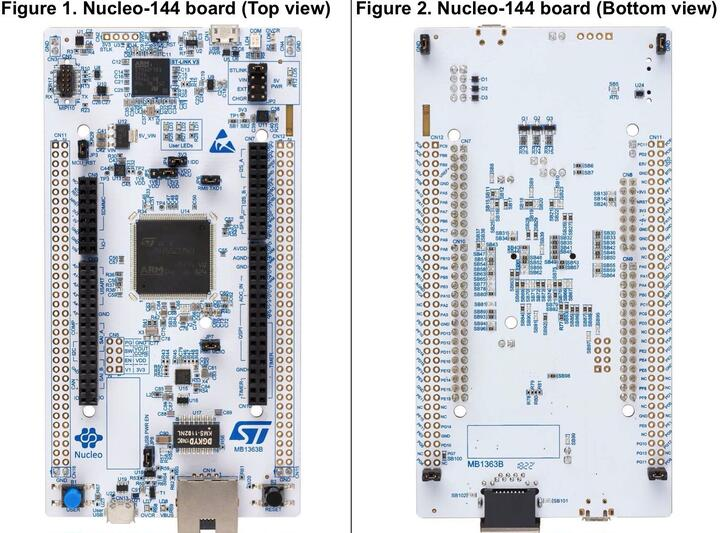
\includegraphics[width=.9\columnwidth]{figures/nucleo.png}
    \caption{Nucleo-144 board both sides }
    \label{fig:1}
\end{figure}

\newpage
\subsection{CubeMX}
STM32CubeMX is a free, cross-platform desktop application from STMicroelectronics that turns the entire bring-up of an STM32 board into a guided, point-and-click workflow.
The graphical interface allows an easy configuration of STM32 microcontrollers and microprocessors, as well as the generation, through a step-by-step process, of the corresponding C initialisation code for 32-bit ARM Cortex STM32 microcontrollers.
The interface provides the means to configure pin assignments, clock tree, integrated peripherals and simulate the power consumption of the resulting project. It uses a rich library from the STM32 microcontroller portfolio.
For microprocessors, it configures the General-Purpose Input/Outputs (\gls{GPIO}s), performs the clock setup for the whole system, and interactively assigns the peripherals.
For microcontrollers and microprocessors built on the Arm Cortex-M core, CubeMX adds helpers such as a pinout-conflict solver, a clock-tree setting helper, a power-consumption calculator, and a utility that configures the peripherals (such as \gls{GPIO} or USART) and the middleware stacks (such as USB or TCP/IP).
The conflict solver checks that no two functions share the same pin. 

\begin{figure}[h]
    \centering
    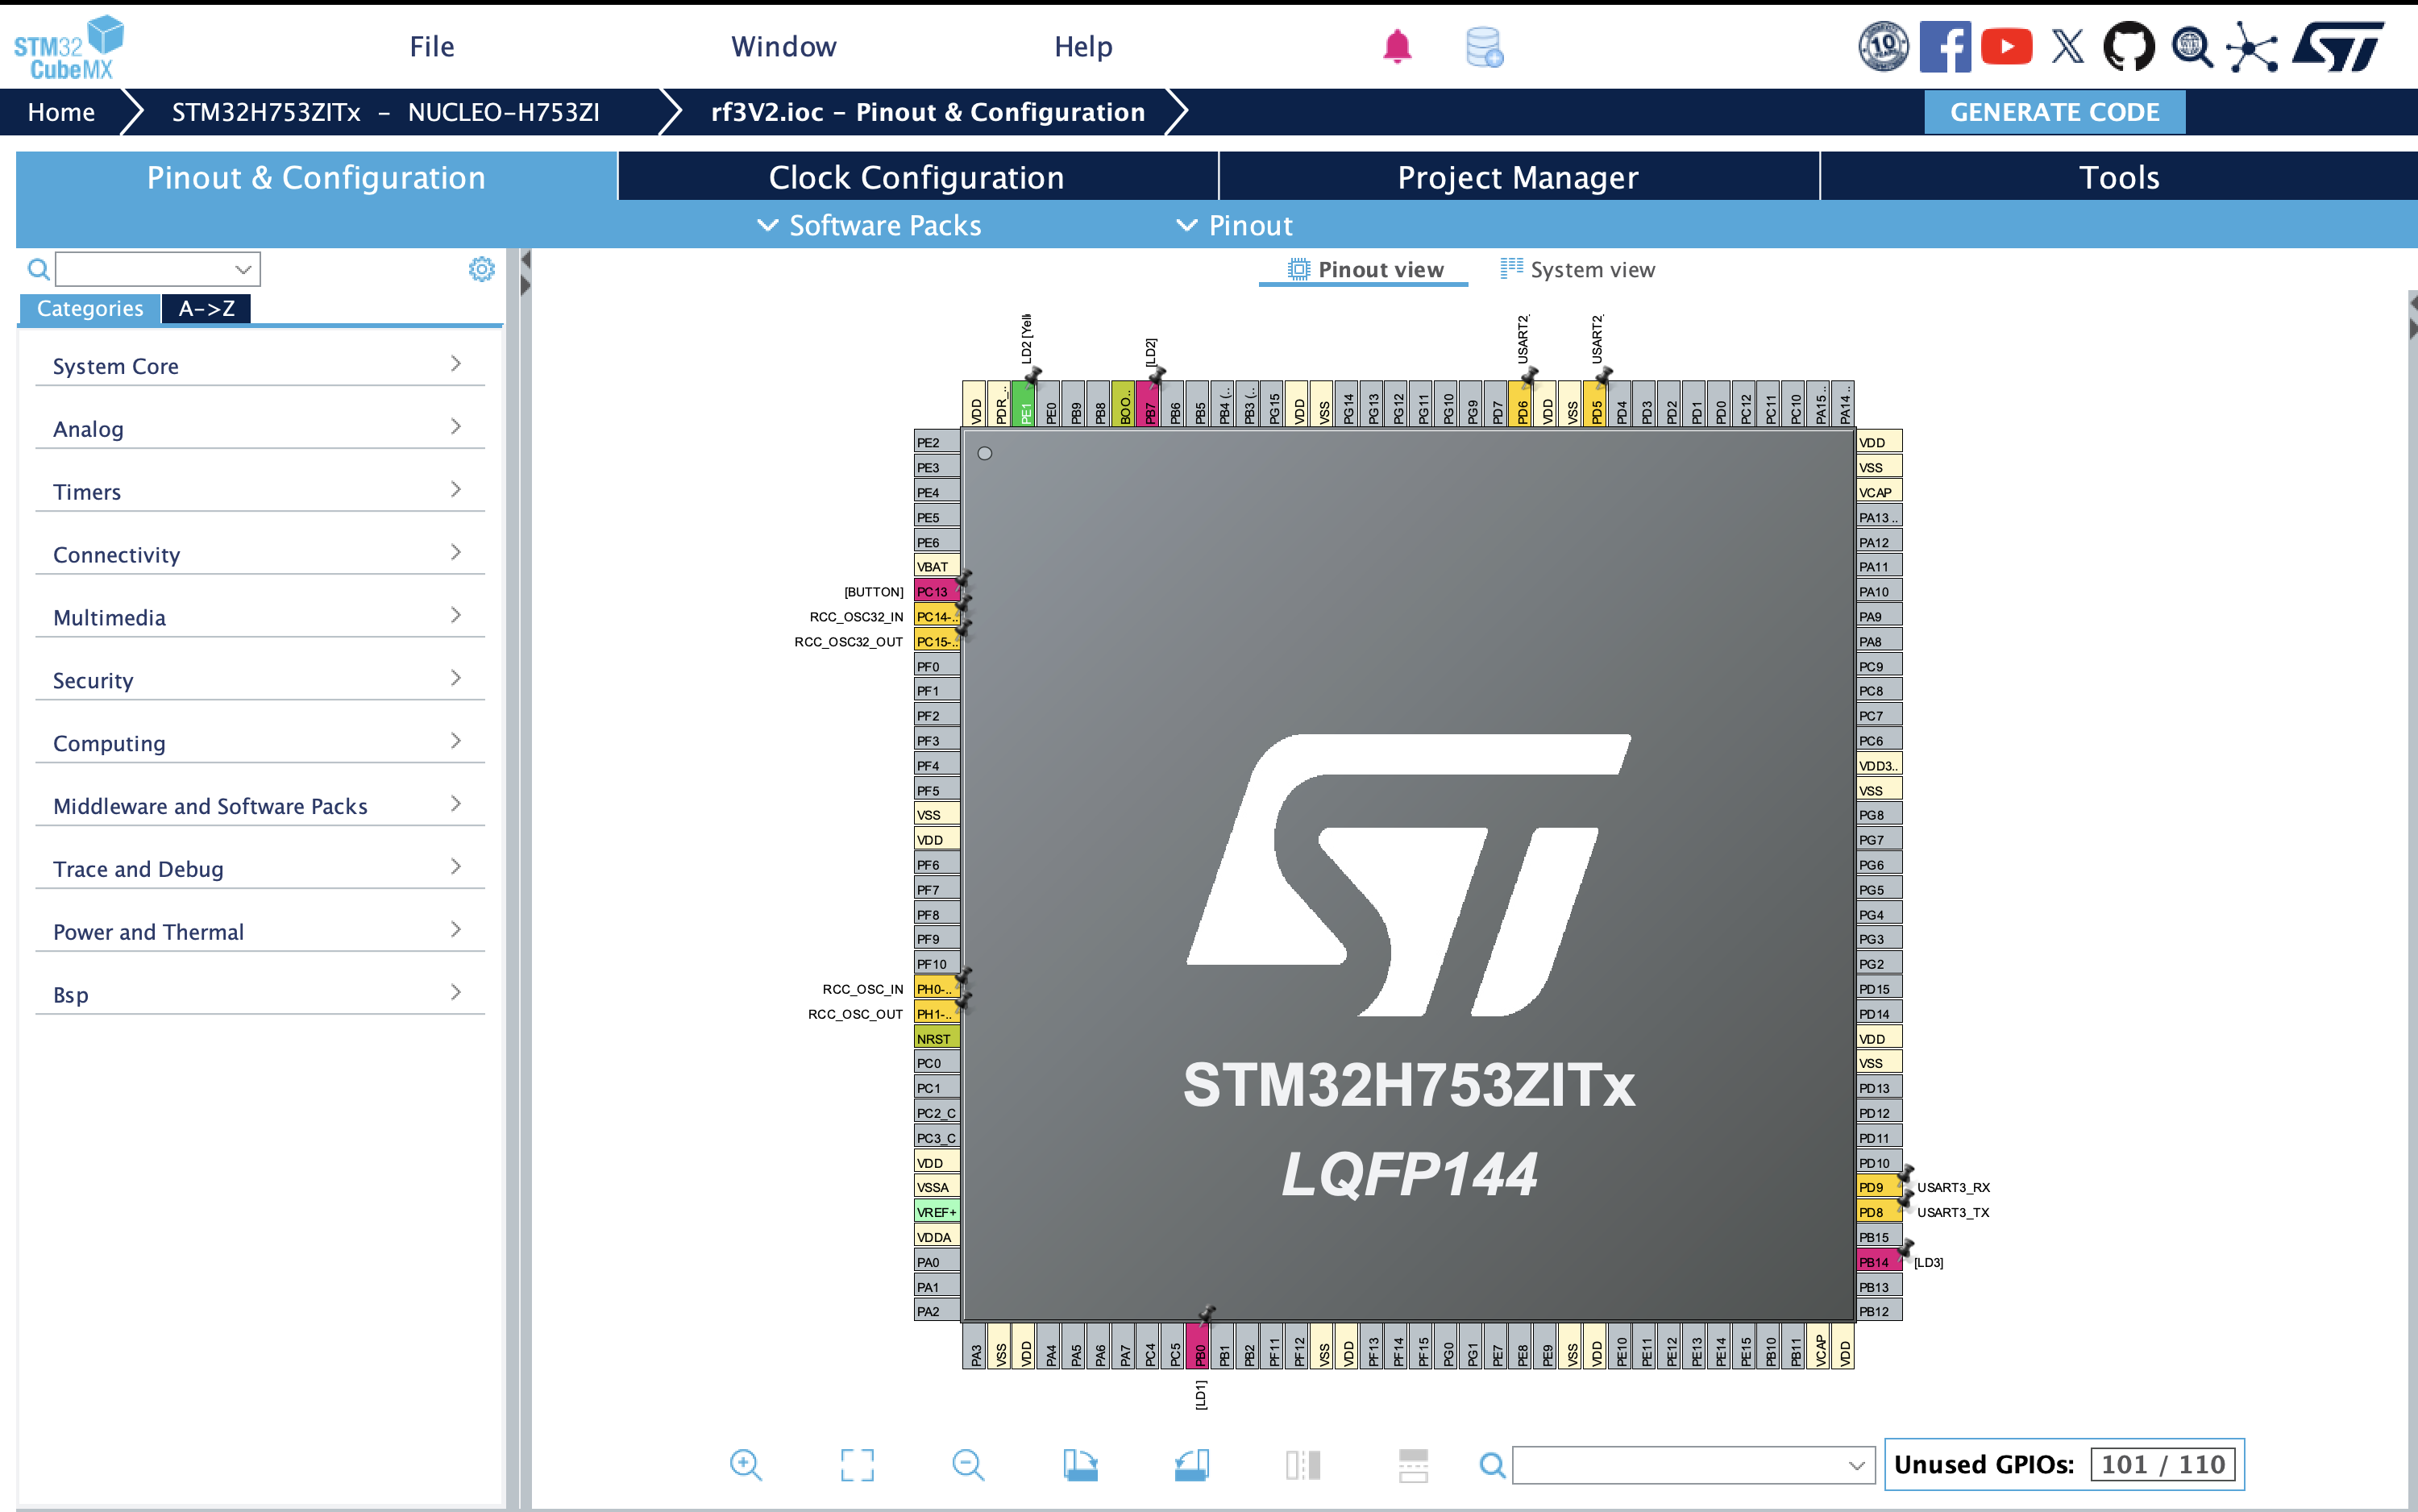
\includegraphics[width=.9\columnwidth]{figures/Cubemx.png}
    \caption{CubeMX application}
    \label{fig:2}
\end{figure}

\subsection{Minicom}
Minicom serves as the primary software for serial communication terminals, used for interfacing with microcontroller hardware. It is a Linux-based terminal emulator that provides a reliable communication channel between the development host system and the target hardware via serial connections such as \gls{UART}. For devices without displays, like switches, routers, or server blade enclosures, one can use Minicom to create a console. 


We chose to use Minicom for the following reasons: 
\begin{enumerate}
  \item Cross-platform compatibility: It is cross-platform with multiple operating systems, such as Linux systems and macOS.
  \item Cost-effective: Minicom is a free-to-use and free-to-install software that requires no additional purchases.
  \item Real-time communication: Provides immediate, bidirectional communication with the target hardware without buffering delays
\end{enumerate}
\TODO{ADD SOURCES}

\subsection{HAL and BSP}

\subsubsection{HAL}

\gls{HAL} is a firmware-level abstraction that sits between the application code and the \gls{MCU} registers. It exposes a uniform C \gls{API} and generates functions. \gls{HAL} works by providing a set of standardised functions and protocols that abstract the low-level details of hardware devices. Through the use of a high-level application programming interface (\gls{API}), this abstraction enables software applications to interact with hardware devices. We chose \gls{HAL} because it offers several benefits, including the fact that one \gls{API} covers \gls{GPIO}, \gls{UART}, SPI, I²C, timers, DMA, ADC, etc. Furthermore, \gls{HAL} simplifies software development by providing a consistent and well-defined interface for interacting with hardware devices. By providing a single, high-level \gls{API} for \gls{UART}, \gls{GPIO}, and timers, the \gls{HAL} lets us implement our error-detection routines once and run them identically on both microcontrollers, thus ensuring consistent timing and data integrity without hand-tuning hardware registers. \TODO{ADD SOURCES}

\subsubsection{BSP}
\gls{BSP} is a special set of tools made just for a specific hardware setup. It helps connect the hardware to the operating system in an embedded system. Its main job is to provide the software and drivers needed so that the OS can communicate appropriately with the hardware. Additionally, the \gls{BSP} includes information about the kernel configuration and hardware features. A \gls{BSP} consists of several components, such as a boot loader, \gls{HAL}, peripheral libraries, and device drivers. Implementing the \gls{BSP} in our project was very helpful as the \gls{BSP}'s board-specific initialisation and driver layer guaranteed that each board came up with the correct clocks, pinmux, and peripheral settings every time, eliminating unpredictable bring-up issues and enabling reliable error-signal exchange.\TODO{ADD SOURCES}


\newpage

\section{Set up}
Detailed description of the toolchain that is required to complete the task.
Describe how to install the required drivers/software/..., how to set up the environment to work with devices, etc.

\TODO{extend including pictures/block diagrams, etc. and more subsections}

\TODO{min. 1-2 pages}

\subsection{Hardware Configuration}
\subsubsection{Board Preparation}
Our communication system requires two NUCLEO-H753ZI development boards, which are both connected to the same laptop via a USB cable. These USB cables must be connected to the top Micro-B USB port to ensure the following purposes:
\begin{itemize}
\item Provides power supply to the development boards
\item Allows programming and flashing through the integrated ST-LINK/V2-1 debugger
\item Creates a virtual COM port for serial communication monitoring
\item Allows debugging
\end{itemize}
Both boards can operate independently while maintaining USB connectivity to the same laptop, allowing for simultaneous monitoring and control of both transmission and reception.

\subsubsection{Inter-Board Communication}
The physical communication link between the two development boards requires establishing a \gls{UART} connection using jumper wires. Using the board instructions, we established three jumper wire connections like the following:
\begin{itemize}
\item Transmit to receive cross-connection: (maybe umschreiben/ändern)
    \begin{itemize}
    \item Board 1 TX (PD5) to Board 2 RX (PD6)
    \item Board 2 TX (PD5) to Board 1 RX (PD6)
    \end{itemize}
\item Common Ground:
    \begin{itemize}
    \item Board 1 GND to Board 2 GND
    \end{itemize}
\end{itemize}
For our project, we use USART 2  through the ZIO connector CN9 for inter-board connection on each board:
\begin{itemize}
\item TX pin (PD5): available on connector CN9, pin 6
\item RX pin (PD6): available on connector CN9, pin 4
\end{itemize}
This setup ensures that either board can function as the transmitter or the receiver, allowing both boards to communicate with each other. 

\subsubsection{Communication Interface}
For inter-board communication, both development boards utilise USART2 while simultaneously maintaining USART3 for USB communication with the laptop. With this configuration, we ensure that the transmitter board receives data from the laptop via USART3, which is then processed through error correction encoding and transmitted via USART2. The receiver board, on the other side, receives data via USART2 and performs error detection and correction. After that, the board sends the result to the laptop via USART3.
The dual \gls{UART} configuration enables real-time monitoring of both the transmission and reception processes from our laptop, allowing us to perform debugging and performance analysis.

\begin{figure}[h]
    \centering
    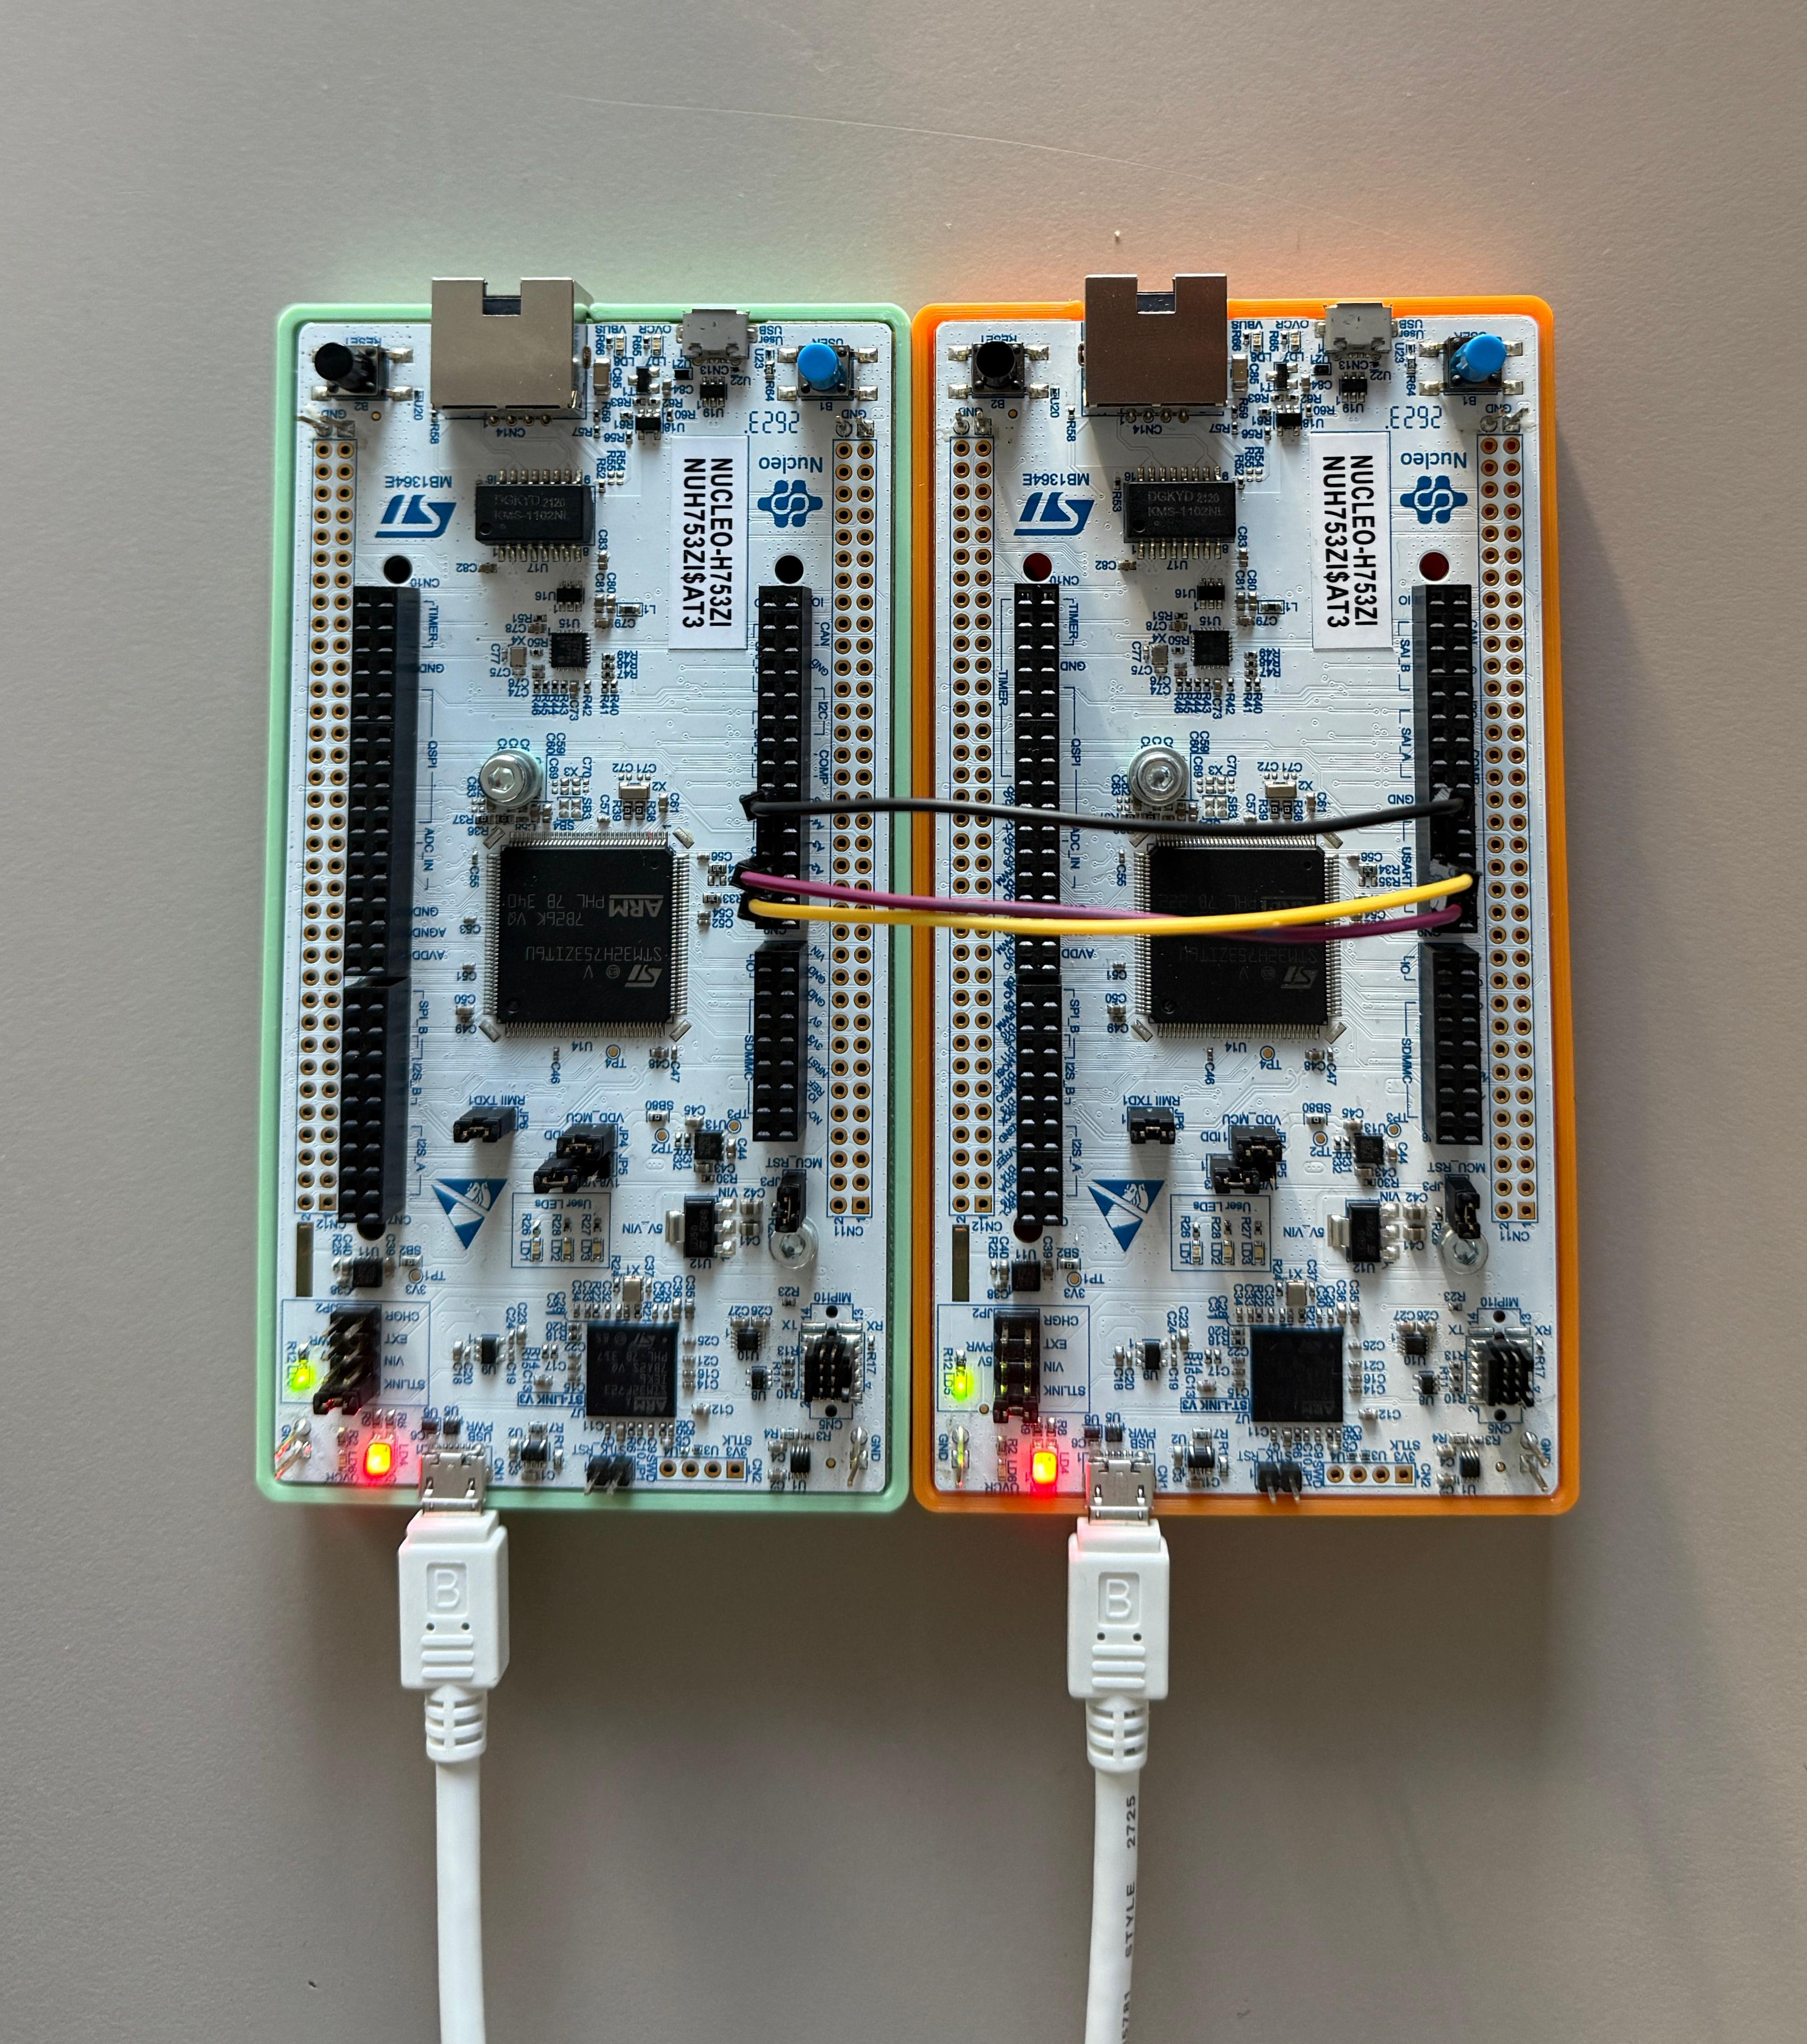
\includegraphics[width=.7\columnwidth]{figures/BOARD SET UP.png}
    \caption{\gls{MCU}s connected}
    \label{fig:3}
\end{figure}

\subsection{UART Parameters}
For the \gls{UART} parameters, we chose the standard configuration (115200-8-N-1), which must be identical for all \gls{UART} interfaces within the system:
\begin{itemize}
\item Baud Rate: 115200 bps
\item Data Bits: 8
\item Parity: None
\item Stop Bits: 1
\item Flow Control: None
\end{itemize}

The virtual COM of each board operates independently, allowing simultaneous communication with both boards from a single laptop.

\subsection{Dual Terminal Minicom}
Our system requires two separate terminal sessions running simultaneously on the laptop, each connected to one of the boards. This dual-terminal setup enables us to monitor input/output data, error correction and detection, as well as transmission status.


\newpage


\section{Error Handling Codes}

\TODO{CRC32-WHY WE USED IT AND WHAT IT IS}

\newpage

\section{Results}
Detailed description and discussion of your results (either positive or negative).

\TODO{extend including pictures/block diagrams, etc. and more subsections}

\TODO{min. 2 pages}

\newpage

\section{Summary}
Summary of the entire document's contents, from motivation to results.

\TODO{max. 1 page}

\end{document}3

